% !TEX TS-program = pdflatex
\documentclass[11pt,a4paper,english]{article}
\usepackage[utf8]{inputenc}
\usepackage[T1]{fontenc}
\usepackage[obeyspaces, hyphens]{url}
\usepackage[top=4cm, bottom=4cm, left=3cm, right=3cm]{geometry}
\usepackage{enumerate}
\usepackage{amsmath}
\usepackage{mdwlist}
\usepackage{fancyhdr}
\usepackage{cite}
\usepackage{amsmath}
\usepackage[normalem]{ulem} % ulem enables strikethrough and more, but makes
                            % \emph underline by default :(
\usepackage{babel}
\usepackage{fancyvrb}
\usepackage{verbatimbox}
\usepackage{amsfonts}
\usepackage{amsthm}
%\usepackage{minted}
\usepackage{xcolor}
\usepackage{csquotes}
\usepackage{listings}
\usepackage{graphicx}
\usepackage{caption}
\usepackage{subcaption}
\usepackage{booktabs}
\usepackage{csquotes}
\usepackage{array}
\usepackage{lmodern} % better font
\usepackage[noend]{algpseudocode}
\usepackage{algorithm}
\usepackage{tikz}
\usepackage{paralist}
\usepackage[font=footnotesize,labelfont=bf]{caption}
\usetikzlibrary{arrows, decorations.markings}
\usepackage{hyperref} % always load hyper ref in the end
\usepackage{cleveref} % except cleveref
\newcolumntype{P}[1]{>{\centering\arraybackslash}p{#1}}

\newcommand*\justify{%
  \fontdimen2\font=0.4em% interword space
  \fontdimen3\font=0.2em% interword stretch
  \fontdimen4\font=0.1em% interword shrink
  \fontdimen7\font=0.1em% extra space
  \hyphenchar\font=`\-% allowing hyphenation
}

\lstset{
    frame=lrtb,
    captionpos=b,
    belowskip=0pt
}

\captionsetup[listing]{aboveskip=5pt,belowskip=\baselineskip}

\newcommand{\todo}[1]{\textcolor{red}{\textbf{TODO: }#1}}

%\definecolor{lightgray}{rgb}{0.95,0.95,0.95}
%\renewcommand\listingscaption{Code}

\newcommand{\concat}{\ensuremath{+\!\!\!\!+\!\!}}

\pagestyle{fancy}
\headheight 35pt

\DefineVerbatimEnvironment{code}{Verbatim}{fontsize=\small}
\DefineVerbatimEnvironment{example}{Verbatim}{fontsize=\small}
\newcommand{\ignore}[1]{}

\hyphenation{character-ised}

\rhead{Assignment 2}
\lhead{ACS}
\begin{document}

\thispagestyle{empty} %fjerner sidetal
\hspace{6cm} \vspace{6cm}
\begin{center}
\textbf{\Huge {Advanced Computer Systems}}\\ \vspace{0.5cm}
\Large{Assignment 2}
\end{center}
\vspace{3cm}
\begin{center}
\Large{\textbf{Truls Asheim, Rasmus Wriedt Larsen, Viktor Hansen}}
\end{center}
\vspace{6.0cm}
\thispagestyle{empty}

\newpage

\section{Exercises}

\subsection{Serializability \& Locking}

\subsubsection{Scenario 1}

\begin{figure}[H]
\centering
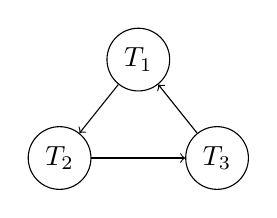
\begin{tikzpicture}
  \node[draw,circle] (t1) at (0,0) {$T_1$};
  \node[draw,circle] (t2) at (-1,-1.25) {$T_2$};
  \node[draw,circle] (t3) at (1,-1.25) {$T_3$};

  \draw [->] (t1) -- (t2);
  \draw [->] (t2) -- (t3);
  \draw [->] (t3) -- (t1);
\end{tikzpicture}
\end{figure}

%T1 precedes T2 (because of X)
%T2 precedes T3 (because of Z)
%T3 precedes T1 (because of Y)

As there is a cycle in the precedence graph, the schedule is \emph{not} conflict-serializable.

This schedule could not have been generated by strict two-phase locking
(non-conservative). The reason is \texttt{T1} will aquire a shared lock on
\texttt{X} initially, so \texttt{T2} will need to wait for \texttt{T1} to
commit, before it can get an exclusive lock on \texttt{X} for \texttt{W(X)}.

\subsubsection{Scenario 2}


\begin{figure}[H]
\centering
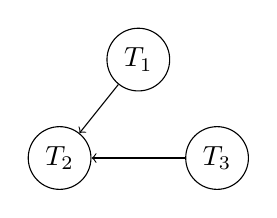
\begin{tikzpicture}
  \node[draw,circle] (t1) at (0,0) {$T_1$};
  \node[draw,circle] (t2) at (-1,-1.25) {$T_2$};
  \node[draw,circle] (t3) at (1,-1.25) {$T_3$};

  \draw [->] (t3) -- (t2);
  \draw [->] (t1) -- (t2);
\end{tikzpicture}
\end{figure}

%T3 precedes T2 (because of Z)
%T1 precedes T2 (because of Y and X)

As there is no cycles in the precedence graph, the schedule is conflict-serializable.

This schedule could be generated by strict two-phase locking (non-conservative),
as illustrated below.

\begin{verbatim}
T1: S(X)                            X(Y)  c
T2:                    S(Z)                       X(X) X(Y) C
T3:        X(Z)   C
\end{verbatim}

\subsection{Questions 2: Optimistic Concurrency Control}
In the Kung-Robinson optimistic concurrency model, we have to consider
intersections of overlapping read and write sets, $R_{i}$ and $W_{i}$
respectively, for all transactions $T_{i}$. A non-empty intersection
semantically corresponds to possible Read After Write (RAW), Write After Read
(WAR) and Write After Write (WAW) conflicts/dependencies, i.e. if the same
location is accessed by two different transactions and at least one of the
accesses is a write.


\paragraph{Scenario 1}
We will consider the intersection of all read and write sets that involve
$T_{3}$, with a few restrictions. We know that \begin{inparaenum}[1)] \item
  $T_{1}$ completes before
$T_{3}$ begins with its write phase and \item $T_{2}$ completes read phase before
$T_{3}$ does.\end{inparaenum} This means $R_{1} \cap W_{3} = \emptyset$,
$W_{1} \cap R_{3} = \emptyset$, $W_{1} \cap W_{3} = \emptyset$ and
$R_{2} \cap W_{3} = \emptyset$, $W_{2} \cap W_{3} = \emptyset$ as these
read/write sets are guaranteed to not overlap. The intersections are depicted in
Table \ref{tbl:scenario1}:
\begin{table}[!hbt]
\centering
\begin{tabular}{|c|c|c|c|}
\hline
$\cap$  & $W_{1}$ & $W_{2}$ & $W_{3}$    \\ \hline
$R_{1}$ & x  & x  & $\emptyset$ \\ \hline
$R_{2}$ & x  & x  & $\emptyset$ \\ \hline
$R_{3}$ & $\emptyset$ & $\left\{ 4 \right\}$ & x \\ \hline
$W_{1}$ & x  & x  & $\emptyset$ \\ \hline
$W_{2}$ & x  & x  & $\emptyset$ \\ \hline
$W_{3}$ & $\emptyset$ & $\emptyset$ & x \\ \hline
\end{tabular}
\caption{Intersections of all $R_{i}$ and $W_{i}$ that overlap and involve $T_{3}$.}
\label{tbl:scenario1}
\end{table}

There is an overlap between the read set of $T_{3}$ and the write set of $T_{2}$ on element $4$, so $T_{3}$ will have to abort.

\paragraph{Scenario 2} In this case, it is given that \begin{inparaenum}[1)]
\item $T_{1}$ completes before $T_{3}$ begins its write phase and \item $T_{2}$
  completes its read phase before $T_{3}$ begins its read phase.\end{inparaenum} This means that
$W_{1} \cap W_{3} = \emptyset$, $R_{1} \cap W_{3} = \emptyset$,
$R_{2} \cap W_{3} = \emptyset$,
\begin{table}[!hbt]
\centering
\begin{tabular}{|c|c|c|c|}
\hline
$\cap$  & $W_{1}$ & $W_{2}$ & $W_{3}$    \\ \hline
$R_{1}$ & x  & x  & $\emptyset$ \\ \hline
$R_{2}$ & x  & x  & $\emptyset$ \\ \hline
$R_{3}$ & $\left\{ 3 \right\}$ & $\emptyset$ & x \\ \hline
$W_{1}$ & x  & x  & $\emptyset$ \\ \hline
$W_{2}$ & x  & x  & $\emptyset$ \\ \hline
$W_{3}$ & $\emptyset$ & $\emptyset$ & x \\ \hline
\end{tabular}
\caption{Intersections of all $R_{i}$ and $W_{i}$ that overlap and involve $T_{3}$.}
\label{tbl:scenario1}
\end{table}

In the case, $T_{1}$ writes element $3$ after $T_{3}$ has read element $3$,
$T_{3}$ a RAW dependency is violated. In this case, $T_{3}$ will have to perform a rollback.

\paragraph{Scenario 3}
In this final case, we know that \begin{inparaenum}[1)] \item $T_1$ completes before
  $T_3$ starts its write phase and that \item $T_2$ completes before $T_3$
  starts its write phase \end{inparaenum}. All of the intersections between the
read and write sets can be seen in \Cref{tbl:scenario3}.

\begin{table}[!hbt]
\centering
\begin{tabular}{|c|c|c|c|}
\hline
$\cap$  & $W_{1}$ & $W_{2}$ & $W_{3}$    \\ \hline
$R_{1}$ & x  & x  & $\emptyset$ \\ \hline
$R_{2}$ & x  & x  & $\{7,8\}$ \\ \hline
$R_{3}$ & $\emptyset$ & $\emptyset$ & x \\ \hline
$W_{1}$ & x  & x  & $\emptyset$ \\ \hline
$W_{2}$ & x  & x  & $\emptyset$ \\ \hline
  $W_{3}$ & $\emptyset$ & $\emptyset$ & x \\ \hline
\end{tabular}
\caption{Intersections of all $R_{i}$ and $W_{i}$ that overlap and involve $T_{3}$.}
\label{tbl:scenario3}
\end{table}

As it can be seen, the only potential conflicts are between $R_2$ and $W_3$, but
since $T_2$ completes before $T_3$ starts its write phase its WAR dependency
isn't violated. Thus, $T_3$ can commit.

\section{Programming Assignments}
\subsection{Tests}
\subsubsection{Test 1 --- Fixed number of parallel buys and adds}
In this test we run two clients, $C_1$ and $C_2$ both of which operates on the
same set of books. $C_1$ buys books while $C_2$ re-adds the same number of
copies. The two clients perform a fixed number of results in parallel. The test
is successful if the number of copies in the book store is the same before and
after the test has run.

The purpose of the test is to check the all-or-nothing semantics of {\tt
  buyBooks} and {\tt addCopies}. If either a buy or an add operation only
completes partially the number of books will be left in an incomplete state and
will thus never 

\subsubsection{Test 2 --- }
The purpose of this test is to check that the all-or-nothing semantics of the
buyBooks and 

\subsection{Test 3 --- }

This test is a variation of the first test except that queries originate from
1000 different clients instead of just 2

\subsection{Questions for Concurrent Implementation of Bookstore}
\subsubsection{Description of Implementation}
The locking protocol was implemented with a single \texttt{ReentrantReadWriteLock}\footnote{\url{http://docs.oracle.com/javase/6/docs/api/java/util/concurrent/locks/ReentrantReadWriteLock.html}} implementing the  \texttt{ReadWriteLock}\footnote{\url{http://docs.oracle.com/javase/6/docs/api/java/util/concurrent/locks/ReadWriteLock.html}}. The JavaDoc for the \texttt{ReadWriteLock} interface  states:

\begin{displayquote}
A ReadWriteLock maintains a pair of associated locks, one for read-only operations and one for writing. The read lock may be held simultaneously by multiple reader threads, so long as there are no writers. The write lock is exclusive.

All ReadWriteLock implementations must guarantee that [...] a thread successfully acquiring the read lock will see all updates made upon previous release of the write lock.
\end{displayquote}
Methods exhibiting behavior semantically corresponding to reads acquire the read lock (shared lock) before reading and releases it afterwards. This read lock non-blocking for multiple readers. Methods exhibiting write-like behavior acquire the write lock (exclusive lock).
\begin{enumerate}[(a)]
\item Before-or-after atomicity is achieved by using a 
\item{Answer here!}
\end{enumerate}

\subsubsection{Correctness of Locking Protocol}
\subsubsection{Deadlock Occurrence}
In order for a deadlock to occur, we need to acquire a lock which is never
released. For this to happen, a thread of execution must exit abnormally before
it gets a chance to release all of the locks that it has acquired.

In our implementation, we handle the first situation by 
\subsubsection{Scalability}
\subsubsection{Locking Overhead}


\end{document}

%%% Local Variables:
%%% mode: latex
%%% TeX-master: t
%%% End:
